\chapter{Avant de commencer}

\section{Installation et configuration}
\label{sec:Installation et configuration}

Pour pouvoir lancer un site web Django vous aurez besoin d'installer: \newline

\begin{itemize}
    \item \textbf{Python 2.7} ou Python 2.8, à partir de
    \url{https://www.python.org/downloads/}
    \item \textbf{pip} (un installateur de module python), à partir de
    \url{https://pip.pypa.io/en/stable/installing/#install-pip}
    \item \textbf{Django}, avec la commande \verb#pip install Django#
\end{itemize}

Afin de pouvoir lancer et utiliser notre implémentation, il est nécessaire
d’installer plusieurs librairies. Pour ce faire, il suffit d’ouvrir un terminal
et de lancer les commandes suivantes: \newline

\begin{verbatim}
pip install splinter
pip install geocoder
pip install reportlab
pip install sendgrid-django
pip install selenium
\end{verbatim}

Si vous rencontrez certains problèmes au niveau des permissions pour exécuter
les commandes ci-dessus, il est possible de les exécuter avec un argument
supplémentaire \verb#--user#. \newline

\begin{framed}
Exemple: \newline

\verb#pip install --user splinter#
\end{framed}

Il vous est désormais possible de lancer le site en version locale en vous
rendant, via le terminal, dans le dossier \enquote{ASMAE} (voir
figure~\ref{fig:Dossier ASMAE}) en entrant la commande suivante: \newline

\verb#python manage.py runserver#
\bigskip

La console devrait vous afficher le même message celui sur la
figure~\ref{fig:Message de la console lors du démarrage du serveur}

\begin{figure}[!ht]
    \centering
    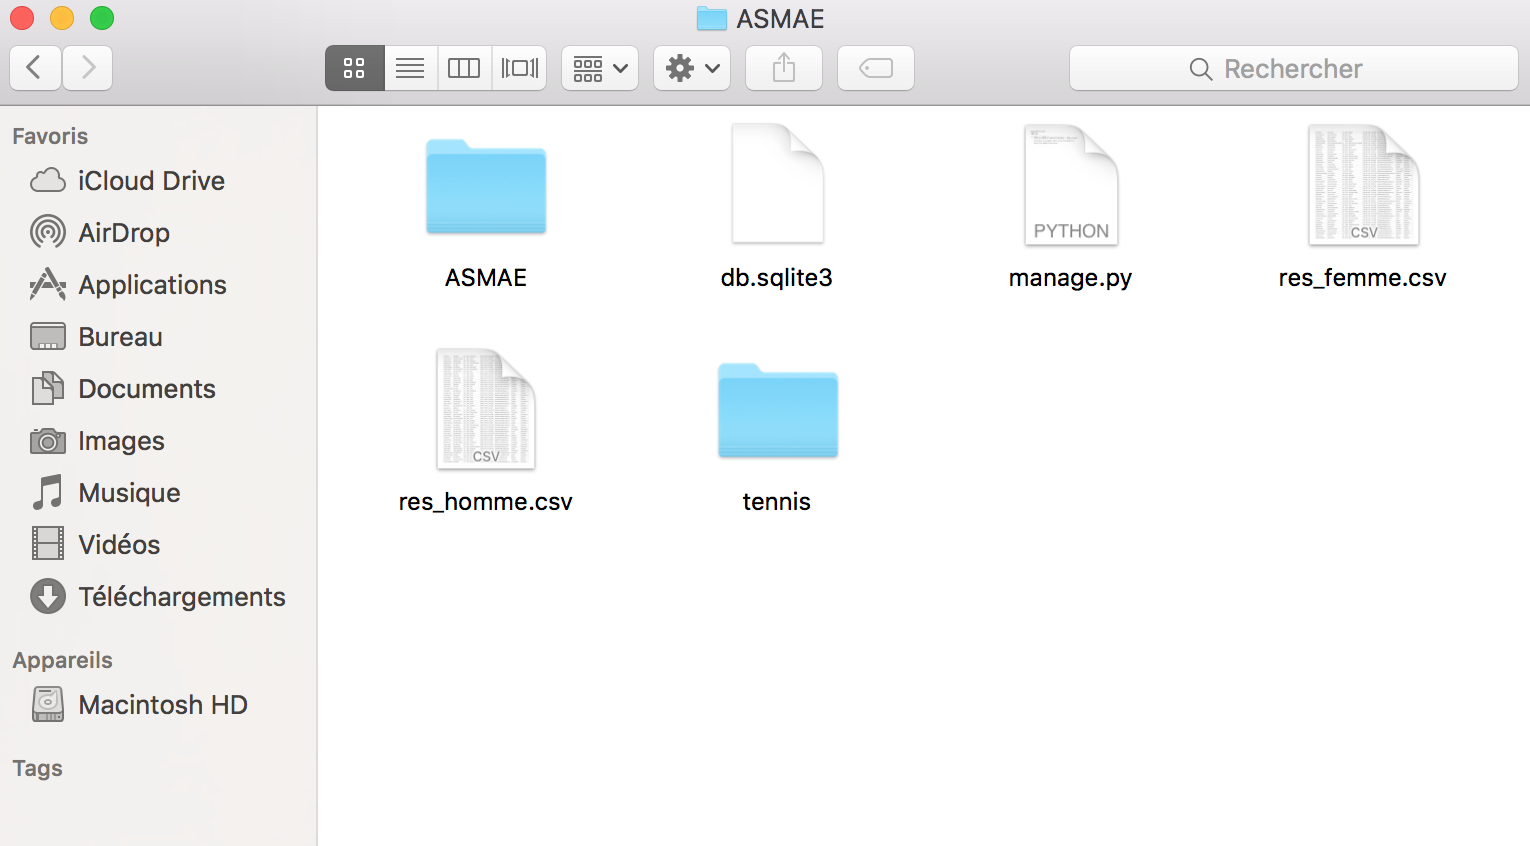
\includegraphics[width=0.5\linewidth]{developer_guide/repertory.png}
    \caption{Dossier ASMAE}
    \label{fig:Dossier ASMAE}
\end{figure}
\FloatBarrier

Il suffit ensuite de lancer le navigateur de votre choix et de vous rendre à
l’adresse suivante : \url{http://localhost:8000/}

\begin{figure}[!ht]
\begin{framed}
\begin{verbatim}
$ python manage.py runserver
Performing system checks...

System check identified no issues (0 silenced).
December 12, 2015 - 20:00:27
Django version 1.8.1, using settings 'ASMAE.settings'
Starting development server at http://127.0.0.1:8000/
Quit the server with CONTROL-C.
\end{verbatim}
\end{framed}
\caption{Message de la console lors du démarrage du serveur}
\label{fig:Message de la console lors du démarrage du serveur}
\end{figure}
\FloatBarrier
